\documentclass[../main.tex]{subfiles}
\begin{document}
\chapter{O CONJUNTO DOS NÚMEROS NATURAIS E OS AXIOMAS DE PEANO}
Neste capítulo apresentaremos os números naturais. Primeiro será apresentada brevemente uma parte histórica e sua importância, após isso, enunciaremos os axiomas. Depois definiremos uma adição, uma multiplicação e uma relação de ordem, bem como listaremos algumas propriedades básicas e faremos suas demonstrações. As referências básicas desse capítulo são \Parencite{domingues-2009} e \Parencite{ferreira}.

\section{Um pouco de história}

Uma possível narrativa para o início do trabalho com números seria à de associação à controle de rebanho por pastores, embora essa narrativa não seja definitiva \Parencite{roque}. Essa iniciação com números e o conhecimento obtido pode ter encontrado dois caminhos (ou fins) possíveis, foram mantidos ao longo do tempo ou não. Nesse sentido não é possível estabelecer uma matemática definitiva e uma única evolução \Parencite[p. 35]{roque}. 

Ao longo da históra, foram desenvolvidos muitos conjuntos numéricos, para resolver problemas que os conjuntos anteriores não eram adequados. 
Com o avanço da matemática, acabou-se esbarrando em problemas que as crenças e técnicas da época não conseguiram resolver, assim uma formalização era necessária, mesmo que não fosse com objetivo de formalizar, mas resolver esses problemas \Parencite[p. 407]{roque}

Quem fundamentou a aritmética como conhecemos hoje foi Giuseppe Peano, mas houve tentativas anteriores, podemos citar Frege. 
Peano conseguiu entre outros fatores por boas escolhas de símbolos, muitos dos quais usamos atualmente, e também por causa da explicitação das regras através de símbolos, e a ausência de hipóteses ocultas \Parencite[p. 415]{boyer}

O trabalho de Peano ficou conhecido como Axiomas de Peano. Ele fundamentou a sua aritmética com 9 axiomas e com 3 conceitos primitivos, como está apresentado na \cref{fig:axiomas-peano}.
\todo{ Referenciar ABNT a figura}
\begin{figure}
    \begin{center}
        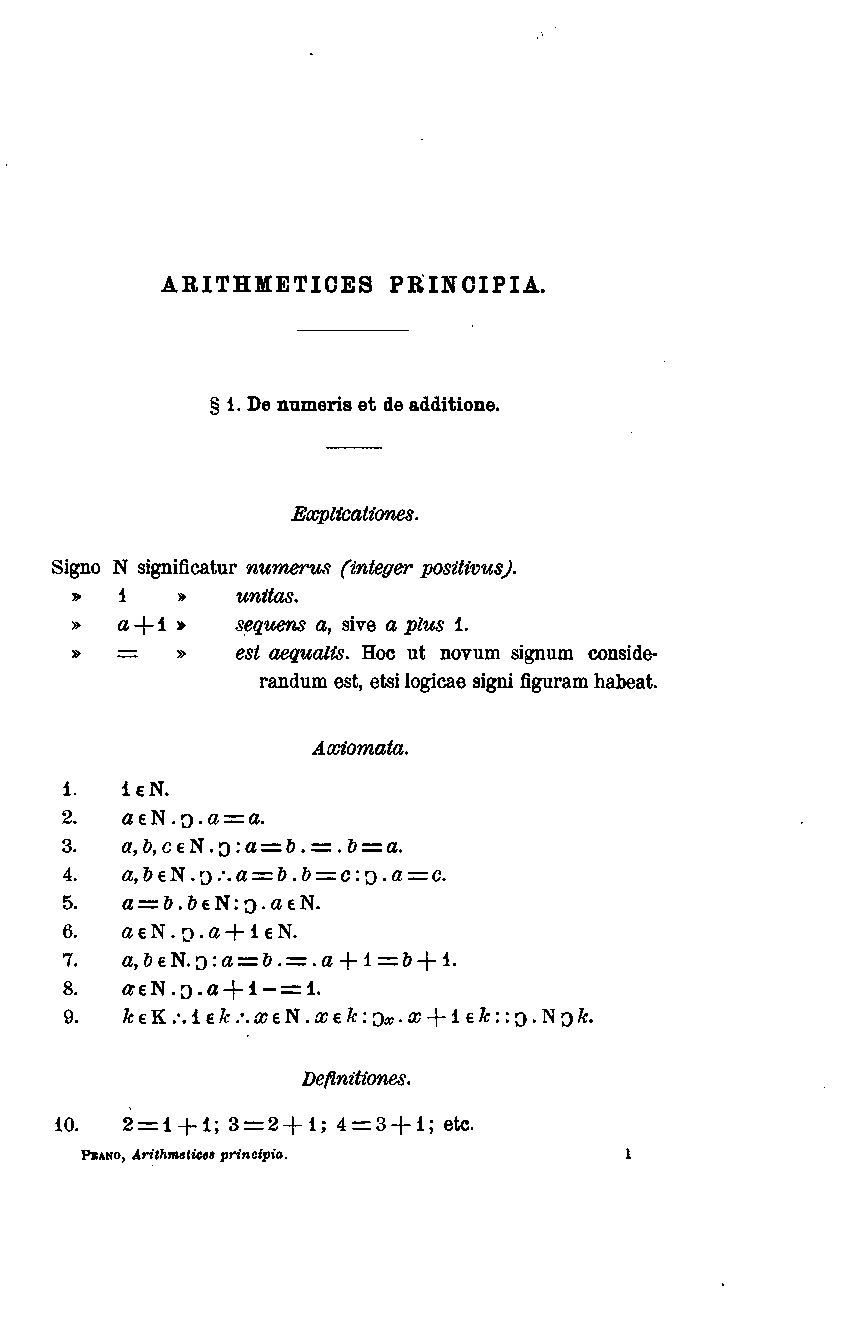
\includegraphics{../include/peano_axioms_original}
        \caption{A versão original dos axiomas de Peano}\label{fig:axiomas-peano}
    \end{center}  
\end{figure}

Antes de continuarmos, podemos recolocar uma analogia da matemática com um jogo:

\begin{displayquote} Ao cirar um jogo, é importante que suas regras sejam suficientes e consistentes. Por \emph{suficiente} queremos dizer que as regras devem estabelecer o que é permitido fazer em qualquer situação que possa vir a ocorrer no desenrolar de uma partida do jogo. Por \emph{consistente} queremos dizer que as regras não devem contradizer-se, ou sua aplicação levar a situações contraditórias. \Parencite[p. 13-14]{barbosa}
\end{displayquote}

Para nós, as peças do jogo serão o conceito de um, o conceito de número natural, e o conceito da relação sucessor. As regras do jogo, naturalmente serão os axiomas que relacionarão esses 3 conceitos primitivos. Nessa analogia, as peças não são muito importantes.

\section{Axiomas}
O nosso estudo dos números naturais será iniciado pela sua apresentação em 3 conceitos primitivos, como os de Peano, e 5 axiomas (ao invés de 9), que são:

\begin{axi}\label{axi-existe-n-s}
    Existe um conjunto de exatamente todos os números naturais, que será denotado por $\N$, e existe uma função $s: \N \rightarrow \N$, que é a relação "sucessor". 
\end{axi}
\begin{axi}\label{axi-um-natural}
    Um é um número natural, isto é, $1 \in \N$.
\end{axi}
\begin{axi}\label{axi-um-nao-sucessor}
    Um não é sucessor de nenhum número, isto é, $1 \not \in Im(s)$ ou ainda, $\not \exists a \in \N : s(a) = 1$.
\end{axi}
\begin{axi}\label{axi-s-injetora}
    $s$ é injetora, isto é, $s(a) = s(b) \implies a = b$ \footnote{Vale notar a contra-positiva que estabelece, nesse caso: $a \neq b \implies s(a) \neq s(b)$}.
\end{axi}
\begin{axi}\label{axi-ind-finita}
    Se $\S$ é um subconjunto de $\N$, caso $1 \in \S$ e se para todo $k$ em $\S\ s(k)$ também esteja em $\S$, então $\S = \N$, isso é o mesmo que colocar: \\
     \[ \S \subseteq \N \land 1 \in S \land ( k \in \S \implies s(k) \in \S) \implies \S = \N .\]
\end{axi}
Este último axioma é chamado de axioma da indução finita.

Conforme os axiomas aprsentados, deve ser notado que o conjunto \N (na nossa axiomatização) não tem o $0$ (zero) que é, usualmente, o neutro da soma em \N. O intuito de construir a partir do $1$ é pela questão que às vezes surge em diversas situações: "$0$ é um número natural?". Em especial, o próprio Lima (2023) diz que o zero pode ser ou pode não ser. É dito que fica a critério de conveniência, embora para nós, seja 'inconveniente' perder o neutro da soma (que aparecerá sua primeira vez em \Z). 

Justificamos essa escolha pois essa dificuldade na ausência do zero terá algumas consequências de reajustes, que poderão ser observadas na nossa construção. Além disso, a bibliografia principal trata o zero como um número natural, então a construção será necessariamente com essas adaptações, o que na visão do autor, é algo positivo para o desenvolvimento do trabalho, mas o resultado final em certo ponto de vista fica prejudicado, pois fica mais "remendado".

Observemos também que o próprio Peano começou originalmente pelo $1$ e somente em trabalho posterior colocou o $0$ como o primeiro número natural.

Para comerçarmos nosso desenvolvimento, podemos notar que o \cref{axi-um-natural} garante $\N \neq \emptyset $. Além dele, o \cref{axi-existe-n-s} garante que $s(1) \in \N$, também $s(s(1)) \in \N$, $s(s(1)) \in \N$ e assim por diante.

Em seguida apresentamos um lema que será necessário para ampliação de nosso ferramental inicial.
\begin{lema}\label{n-dif-sucessor}
    Nenhum número natural é seu próprio sucessor, ou seja, $a \in \N \implies a \neq s(a) $.
\end{lema}
\begin{dem}
    Faremos por indução.\\
    Seja $\S = \{x \in \N : x \neq s(x) \}$
    Os axiomas \ref{axi-um-natural} e \ref{axi-um-nao-sucessor} garantem que $1 \in \S$.\\
    Supondo que existe $ k \in \S$ onde $ k \neq s(k)$, queremos provar que o sucessor de $k$ é diferente do sucessor do sucessor de $k$, isto é, $s(k) \neq s(s(k))$. Como $k \neq s(k)$ e $s$ é injetora pelo \cref{axi-s-injetora}, concluímos que $s(k) \neq s(s(k))$.
\end{dem}
\begin{teo}\label{nat-suc-unico}
    Todo número natural, exceto o $1$ é sucessor de algum outro número natural, que é único.
    % , isto é, $\forall x (x \in \N \land x \neq 1 \implies \exists! y : s(y) = x)$.
\end{teo}
\begin{dem}
    A prova é feita por indução. \\ 
    Seja $\S = \{x \in \N : x \neq 1 \implies (\exists y \in \N \land s(y) = x) \}$.\\
    Sabemos que $1 \in \S$ porque $x = 1$ torna o antecedente falso, assim a implicação é verdadeira. Suponhamos que existe um $k$ em \S, queremos mostrar que $s(k) \in \S$. Devemos observar que $s(k)$ é o sucessor de $k$, assim, colocando na forma que usamos na definição do conjunto,
    $y = k$, $s(y) = s(k)$, dessa forma $s(k) \in \N$. Pelo \cref{axi-ind-finita} temos que \S = \N.

    A unicidade do $y$ que usamos na construção de \S advém do \cref{axi-s-injetora}, $s(z) = s(y) = x \implies z = y$ pela injetividade de $s$.
\end{dem}
\begin{obs}
    Diremos que o número $y$ do teorema anterior é antecessor de $x = s(y)$. Além disso vale notar que $s$ conforme definida no \cref{axi-existe-n-s} não é sobrejetora somente pelo fato de o contradomínio ser \N. Mas se considerarmos o caso restrito para $\N \setminus \{1\}$ 
    teremos que $s$ é uma \emph{bijeção}.
\end{obs}

Faremos a notação usual para os números naturais, isto é, $\N = \{ 1, 2, 3, 4, ...\}$, onde $2 \defeq s(1), 3 \defeq s(2), 4 \defeq s(3)$ e assim por diante.

%%% ADICAO %%%


\section{A adição}
A adição em \N é a que mais intuitivamente está relacionada com a contagem e união de coisas discretas.
\begin{defi}\label{def-adicao-N}
Sejam $a, b \in \N$. A adição entre $a$ e $b$, denotada por $a + b$ é definida com as seguintes condições: 
    \begin{enumerate}[label=(\roman*)]
        \item $a + 1 = s(a)$;
        \item $a + s(b) = s(a+b)$.
    \end{enumerate}
\end{defi}
Às vezes poderemos fazer referência à operação de adição com o nome de soma.

\begin{teo}
    A adição acima é uma função, que leva uma dupla de números naturais em um único número natural.
\end{teo}
\begin{dem}
    A prova de que a soma está bem definida para quaisquer $a,b \in \N$ é dada a seguir:
    Dado $a \in \N$ fixo, seja $\S = \{ x \in \N : a + x \ \text{está definido} \}$. Temos que $a + 1 = s(a)$ está definido, portanto $1$ está em \S. 
    Agora consideremos que vale para um dado $k \in \N$, que $a+k$ esteja bem definida. Temos então que $a + s(k) = s(a+k)$, como $a+k$ está definido, o sucessor também está definido, pelo axioma da indução, temos que \S = \N.
\end{dem}
\begin{lema}\label{soma-n-um-comut}
    O $1$ comuta com qualquer número na soma, isto é,$ \forall x \in \N, x + 1 = 1 + x$
\end{lema}
%       Template
%        Seja $\S = \{ x \in \N : \}$
\begin{dem}
    Seja $\S = \{ x \in \N : x + 1 = 1 + x\}$. O $1$ está em \S pois $1 + 1 = 1 + 1$.
    sabendo que existe um $k$ em \S, queremos provar que $s(k)$ também está em \S. Como
    $s(k) + 1 = s(s(k)) = s(k+1) = s(1+k) = 1 + s(k)$. Portanto $s(k)$ também está em \S sempre que $k$ também está, o que pelo princípio de indução \S = \N.
\end{dem} \\

\begin{prop}{A adição no conjunto dos números naturais tem as seguintes propriedades:}\label{nat-soma-props}
    \begin{enumerate}[label=(\roman*)]
        \item Fechamento;
    	\item Associativa;
    	\item Comutativa;
        \item Lei do cancelamento;
        \item Se $a,b \in \N$, temos $a + b \neq a$;\label{nat-soma-props-distinto}
    	\item Inexistência de neutro: $\not\exists \mathfrak{e} \in \N : \forall a, a + \mathfrak{e} = \mathfrak{e} + a = a$.
    \end{enumerate}
\end{prop}

\begin{dem}
    Antes de demonstrarmos propriamente, façamos a suposição que $a,b,c \in \N$ são números fixos.
    \begin{enumerate}[label=(\roman*)]    
        \item Fechamento: \\
            Seja $\S = \{ x \in \N : a + x \in \N \}$. Obviamente o $1$ está em \S. Suponhamos então que existe $k \in \S$, queremos saber se isso garante que $s(k) \in \S$. Temos então que $a + k \in \N$, já para $a + s(k) = s(a + k) \in \S$, pois pelo \cref{axi-existe-n-s} a função tem domínio e contradomínio \N.
        \item Associativa: \\
             Seja $\S = \{ x \in \N : (a + b) + x = a + (b + x) \}$. Para o $1$ temos então
             $(a + b) + 1 = s(a + b) = a + s(b) = a + (b + 1)$, o que mostra que o $1$ está em \S. 
             Mostraremos que $k \in \S \implies s(k) \in \S$, pois:
             $(a + b) + s(k) = s( (a + b) + k) = s(a + (b + k)) = a + s(b + k) = a + (b + s(k))$, o que, pelo princípio de indução \S = \N.
        \item Comutativa: \\
            Consideremos o conjunto $\S = \{ x \in \N : a + x = x + a\}$. O $1 \in \S$ pois 
            $a + 1 = 1 + a$ conforme o \cref{soma-n-um-comut}.
            Provemos então que se $k \in \S$ então $s(k) \in \S$, temos 
            $a + s(k) = s(a + k) = s(k + a) = k + s(a) = k + a + 1 = k + 1 + a = s(k) + a$.
        \item Lei do cancelamento: \\
            Seja $\S = \{ x \in \N : x + b = x + c \implies b = c \}$, vamos provar que \S = \N. Obviamente o $1$ está em \S pois $1 + b = 1 + c \iff b + 1 = c + 1$ e pelo \cref{axi-s-injetora}, se dois elementos tem sucessores iguais, eles próprios são iguais. Agora consideremos se vale que $(k + b = k + c \implies b = c) \implies (s(k) + b = s(k) + c \implies b = c)$. \\
            $s(k) + b = s(k) + c \iff (k + b) + 1 = (k + c) + 1$, o que pelo mesmo motivo anterior, concluímos que $k + b = k + c$, e pela nossa hipótese concluímos que $b = c$.
        \item $a + b \neq a$;\\
            Consideremos quatro casos:
            \begin{enumerate}[label=(\arabic*)]
            \item $a=1 \land b=1$ \\
                Temos $a+b=a \iff 1+1=1 \absurd$. 
            \item $a=s(x) \land b=1$ \\
                Temos $a+b=a \iff s(x) + 1 = s(x) \iff s(s(x)) = s(x) \absurd$. 
            \item $a=1 \land b=s(y)$ \\
                Temos $a+b=a \iff 1+ s(y) = 1 \iff s(1+y) = 1 \absurd$. 
            \item $a=s(x) \land b=s(y)$ \\
                Temos $a+b=a \iff s(x) + s(y) = s(x) \iff x + 1 + y + 1 = x + 1 \iff s(1 + y) = 1 \absurd$.
            \end{enumerate}
    
        \item Inexistência de neutro: \\
            Como consequência da demonstração anterior, temos que não existe neutro na adição, isto é, $a + \mathfrak{e} = \mathfrak{e} + a = a$.
    \end{enumerate}
\end{dem}
 
Podemos observar que como não existe neutro, não poderemos aplicar descuidadamente as outras propriedades, por exemplo: não poderíamos ter provado que $a \neq a + 1 $ usando a lei do corte e supondo que fossem iguais, assim: $a = a+ 1 \implies 0 = 1$, porque isso não faz sentido no nosso desenvolvimento. Também podemos observar que a lei do cancelamento é independente da \cref{agb-prop-leiCancelamento}, uma vez que não temos neutro.

%%% MULTIPLICACAO %%%
A multiplicação toma seu lugar como uma operação de redução da soma. Essa ideia de notação resumida pode ser explorada quando se faz o uso do sistema posicional, mas não faremos o uso do sistema posicional. 

\section{A multiplicação}
\begin{defi}\label{nat-def-multiplicacao}
    Sejam $a, b \in \N$. A multiplicação entre $a$ e $b$, denotada por $a \cdot b$ é definida com as seguintes condições: 
	\begin{enumerate}[label=(\roman*)]
		\item $a \cdot 1 = a$;
		\item $a \cdot s(b) = a \cdot b + a$.
	\end{enumerate}
\end{defi}

\begin{prop}{Para a multiplicação de números naturais são válidas as seguintes propriedades:}
    \begin{enumerate}[label=(\roman*)]
        \item Fechamento;
        \item Elemento neutro; \footnote{Se for observada a definição de multiplicação, esse número pode ser o $1$}.
        \item Distributiva;
        \item Comutativa;
        \item Associativa;
        \item Lei do cancelamento;
        \item Para $a,b \in N$ ocorre que, $a \cdot b = 1 \implies a = b = 1$.
    \end{enumerate}
\end{prop}
% template
% Seja $\S = \{ x \in \N : \}$
\begin{dem}
    Antes de demonstrarmos propriamente, façamos a suposição que $a,b,c \in \N$ são números fixos. Provaremos por indução, exceto no último item.
    \begin{enumerate}[label=(\roman*)]
        \item Fechamento: \\
            Seja $\S = \{x \in \N : ax \in \N \}$.
            O $1$ está em \S pois $1 \cdot 1 = 1$. Supondo que é válido $ak \in \N$ para algum $k \in \N$, temos $a \cdot s(k) = ak + a$, como tanto $ak$ quanto $a$ são números naturais, e como a soma é fechada em \N, temos $ak + a \in \N$. Pelo \cref{axi-ind-finita}, \S = \N. 
        \item Elemento neutro: \\
            Seja $\S = \{ x \in \N : 1 \cdot x = x \cdot 1  = x \}$. O $1$ está em \S pois $1 \cdot 1 = 1 \cdot 1 = 1$. Supondo que $k \in \S$ podemos concluir que $s(k) \in \S$?
            Temos $1 \cdot s(k) = 1 \cdot k + 1 = k \cdot 1 + 1 = k + 1 = s(k) = s(k) \cdot 1$. Pelo \cref{axi-ind-finita}, \S = \N.
            
            % \\ Além disso, sejam $e_1, e_2$ dois elementos neutros. Então $e_1 = e_1 \cdot e_2 = e_2 \implies e_1 = e_2$, portanto o neutro é único. Além disso a definição de multiplicação nos diz que é o $1$ quem é o neutro. 
        \item Distributiva à direita: 
            Seja $\S = \{ x \in \N : ( a + b ) x = ax + bx \}$. Temos que o $1 \in \S$ pois $( a + b ) 1 = a + b = a \cdot 1 + b \cdot 1$. Provemos que se $k \in \S$ temos que $s(k) \in \S$. Temos então: \\
            $( a + b ) \cdot s(k)= ( a + b ) k + ( a + b ) = ak + bk + a + b = ak + a + bk + b 
            = a \cdot s(k) + b \cdot s(k)$. Pelo \cref{axi-ind-finita} tem-se que \S = \N.
            \\ \\
            Distributiva à esquerda: \\
            A prova da distributiva à esquerda é facilmente obtida quando já dispusermos da propriedade comutativa. Por sua vez a prova da comutatividade que faremos precisará apenas da distributiva à direita.
            % Seja $\S = \{ x \in \N : x (a+b) = xa + xb\} $. O $1 \in \S$ pois ele é o neutro, que comuta com qualquer número, assim temos 
            % $1 \cdot (a+b) = (a+b) \cdot 1 = a + b = a \cdot 1 + b \cdot 1 = 1 \cdot a + 1 \cdot b$. Supondo que vale para algum $k \in \N$, que $k(a+b) = ka + kb$, teremos então que $s(k) \cdot (a+b) = (k+1) \cdot (a+b) = k(a+b) + 1(a+b) = (ka + kb) + (a+b) = ka + a + kb + b = 
            % a \cdot s(k) + b \cdot s(k)$, e pelo \cref{axi-ind-finita} concluímos que \S = \N.
        \item Comutativa: \\
            Seja $\S = \{ x \in \N : ax = xa \}$. Com certeza o $1$ está em \S, porque $1$ é o neutro da multiplicação. Agora suponhamos que $k \in \S$, vejamos se $s(k) \in \S$. Temos então: $a \cdot s(k) = ak + a = 1 \cdot a + ka = (1+k)a = s(k) \cdot a$. Pelo \cref{axi-ind-finita} tem-se que \S = \N.

        \item Associativa:  \\
            Seja $\S = \{ x \in \N : a(bx) = (ab)x \}$. Sabemos que o $1$ está em \S pois $a (b \cdot 1) = a(b) = ab = (ab)\cdot 1$.
            Agora suponhamos que exista um $k \in \S$, assim, podemos omitir parênteses em $abx$ , consideremos $s(k)$, para ver se ele está ou não em \S. Temos
            $a(b \cdot s(k)) = a(bk + b) = abk + ab = s(k) \cdot  (ab)$, o que pelo \cref{axi-ind-finita} tem-se que \S = \N. 
            
            
            
        \item Lei do cancelamento: \\
            Seja $\S = \{ x \in \N : xb = xc \implies b = c\}$. O $1$ está em \S pois $1b = 1c \implies b = c$. Provemos que $k\in \S \implies s(k) \in \S$. Temos que $s(k) \cdot b = s(k) \cdot c \iff b + bk = c + ck \iff b = c$. Pelo \cref{axi-ind-finita} tem-se que \S = \N.
        \item $a \cdot b = 1 \implies a = b = 1$.
            Consideremos que o $a$ ou o $b$ podem ser igual (ou iguais) a $1$.
            Sem perda de generalidade, seja $a = 1$. Temos que $1 \cdot b = 1 \implies b = 1$ pois $1$ é o elemento neutro. Portanto se $a$ ou se $b$ forem $1$, obrigatoriamente o outro deverá ser, para que a igualdade ocorra.
            Consideremos um último caso, se $a \neq 1$ e $ b \neq 1$. Então existem $c$ e $d$ naturais tais que $a = s(c)$ e $b = s(d)$.
            Assim, $ab=1 \iff (c+1) (d+1) = 1 \implies cd + c + d + 1 = 1 \implies s(cd + c + d) = 1$, o que obviamente não pode ocorrer de acordo com o  \cref{axi-um-nao-sucessor}.
    \end{enumerate}
\end{dem}
% Seja $\S = \{ x \in \N : \}$

Nesse desenvolvimento, as propriedades da multiplicação são semelhantes às que teríamos se tivéssemos tomado o $0$ como número natural. Uma propriedade que essa multiplicação não tem agora é o anulamento, que carece de significado. As propriedades associativa e comutativa já eram presentes na soma. Agora no produto, temos um elemento neutro que não há para a soma, além da distributiva que pode ser aplicada com soma e produto.
Na nossa lei do cancelamento, não precisamos especificar que o termo a ser cancelado é diferente de zero.

%%% A RELACAO DE ORDEM %%%

Até agora dispomos de uma soma e um produto em \N, mas isso ainda não nos possibilita comparar dois elementos de \N. Agora, com intuito de responder à pergunta, qual número vem "antes" ou qual número é "menor", devemos estabelecer uma relação de ordem. 

Reforçamos que existem diferentes relações de ordem num mesmo conjunto, conforme o exemplo que segue à \cref{agb-def-relOrd}.

\section{A relação de ordem}
\begin{defi}\label{def-relOrdem-N}
Sejam $a, b \in \N$. Definiremos a relação $\leq$ entre $a$ e $b$, denotado por $a \leq b$, e diremos que $a$ se relaciona com $b$ através de '$\leq$' quando uma das seguintes situações ocorre:
    \begin{itemize}
        \item $a = b$;
        \item $a + n = b, n \in \N$.
    \end{itemize} 
\end{defi}
\begin{obs}
    Deve ser notado que quando $a \leq b$ uma e apenas uma das seguintes situações pode ocorrer $a = b$ ou $a + n = b, n \in \N$. Isso é devido à \cref{nat-soma-props} item \ref{nat-soma-props-distinto}, que mostra que ambas não podem ocorrer simultaneamente. Já considerando que pelo menos uma situação deve ocorrer, é a totalidade, que será provada no final deste capítulo. 
\end{obs}
\begin{prop}{A relação de ordem em \N tem as seguintes propriedades:}
    \begin{enumerate}[label=(\roman*)]
        \item Reflexiva;
        \item Antissimétrica;
        \item Transitiva;
        \item Tricotomia;
        \item Compatível com adição;
        \item Compatível com multiplicação.
    \end{enumerate}
\end{prop}
\begin{dem}
    Primeiro, suponhamos que $a,b,c,m,n$ são números naturais.
    \begin{enumerate}[label=(\roman*)]
        \item Reflexiva: \\
            É imediato que $a = a \implies a \leq a$.
        \item Antissimétrica, $a \leq b \land b \leq a \implies a=b$: \\
            Se $a=b$ não há nada a provar. Consideremos que sejam diferentes.
            Então $a \leq b \iff b = a + n$ e também, como $b \leq a \iff a = b + m$, substituindo, temos $b = (b+m) + n \implies b = b+r$ para algum $r$ natural, o que não pode ocorrer. % como demonstrado no item XXX etc.
        \item Transitiva $a \leq b \land b \leq c \implies a \leq c$: 
            Vamos considerar 4 casos:
            \begin{enumerate}[label=(\arabic*)]
                \item $a = b = c$ \\
                    Temos $a = c \implies a \leq c$\\
                \item $a = b < c$ \\
                    Temos $ b + n = c \implies a + n = c\implies a \leq c$\\
                \item $a < b = c$ \\
                    Temos $a + n = b = c \implies a \leq c$\\
                \item $a < b < c$ \\
                    Temos $a + m = b \land b + n = c \implies ( a + m ) + n = c \implies a \leq c$
            \end{enumerate}
        \item Tricotomia:
        Vamos provar por indução. \\
        Seja $\S = \{ x \in \N : x = a \lor x < a \lor x > a \}$. Sabemos que o $1 \in \S$ porque, ou ocorre que $a = 1$, ou $a = s(m) = m + 1$, para algum $m$ natural, assim, $1 < a$. \\
        Supondo que vale para algum $k$ que $k = a \lor k < a \lor k > a$, consideremos 3 casos.  \\
        
        No primeiro caso, $k = a$, assim $s(k) > a$. \\
        No segundo caso, $k < a$, assim $k + m = a$, para algum $m$ natural. Se $m = 1$, $k+1 = s(k) = a$. Se por outro lado, $m \neq 1$, então $m = s(n)$ para algum $n$ natural, assim, $a = k + m = k + n + 1 = s(k) + n$, dessa forma $a > s(k)$. \\
        No terceiro caso, $k > a$, assim $k = a + m$ para algum $m$ natural, e $s(k) = a + m + 1 > a$.

        A unicidade, embora não esteja explícita na criação do conjunto, pode ser vista no desenvolvimento de cada caso.
        Portanto, em todos os casos, $s(k) \in \S$, e pelo \cref{axi-ind-finita}, \S = \N.
        
        \item Compatível com adição: \\
        Seja $a \leq b$. Se $a = b$ teremos que $a+c = b+c$ porque a adição é uma função! 
        Consideremos agora $a < b$. Então $b = a + m \implies b+c = a+m+c \implies a+c < b+c$.
        \item Compatível com multiplicação: \\
        É análogo ao caso da compatibilidade com a adição.
     \end{enumerate}
\end{dem}

\begin{corol}\label{nat-coro-tric}
    A relação de ordem $\leq$ definida anteriormente é total. \footnote{Basta observar a tricotomia}
\end{corol}

{ \textoIncluido
\begin{prop}
    Se $a,b,c \in \N$ e $a + c \leq b + c$ então $a \leq b$.
\end{prop}
\begin{dem}
    Se $a + c = b + c$, pela lei do cancelamento para a adição temos $a=b \therefore a \leq b$.
    Se $a + c + m = b + c$, para algum $m$ natural, novamente pelo cancelamento da adição temos $a+m = b$, assim $a < b \therefore a \leq b$.
\end{dem}
\begin{prop}
    Se $a,b,c \in \N$ e $a \cdot c \leq b \cdot c$ então $a \leq b$.
\end{prop}
\begin{dem}
    Se $ac = bc$, pela lei do cancelamento do produto, $a=b \therefore a \leq b$.
    Se por outro lado, $ac < bc$, então $bc = ac + m$, para algum $m$ natural. Mostraremos por contradição, que não pode ocorrer $a > b$.
    Suponhamos que isso ocorra $a > b$, então $ac > bc$, e assim $ac = bc + n$ para algum $n$ natural. Então temos que 
    $bc = ac + m \iff bc = (bc + n) + m$, o que não pode ocorrer pela \cref{nat-soma-props}, $a+b \neq a$. Uma outra demonstração dessa segunda parte seria pela tricotomia, que não permite que ocorra $ac < bc $ e $ac > bc$.
\end{dem}
}

\end{document}